\documentclass[10pt]{article}
\usepackage{tmlr}
% Camera-ready: \usepackage[accepted]{tmlr}; de-anonymized preprint: \usepackage[preprint]{tmlr}

\usepackage[T1]{fontenc}
\usepackage[utf8]{inputenc}
\usepackage{amsmath,amssymb,amsthm}
\usepackage{booktabs}
\usepackage{tabularx}
\usepackage{array}
\usepackage{graphicx}
\usepackage{xcolor}
\usepackage{tikz}
\usetikzlibrary{arrows.meta,positioning,fit,calc,backgrounds}
\usepackage{enumitem}
\usepackage{microtype}
\usepackage{float}
\usepackage{hyperref}
\usepackage{url}
\usepackage[nameinlink,capitalise]{cleveref}

\hypersetup{
  pdftitle={Beating Greedy Is Not Enough: A Preregistered Benchmark for Budgeted Allocation of Certified Entanglement},
  pdfauthor={Anonymous},
  colorlinks=true, linkcolor=blue!50!black, citecolor=blue!50!black, urlcolor=blue!50!black,
  pdfkeywords={reinforcement learning, baselines, preregistration, budgeted allocation, bid prices, benchmark, entanglement},
}

% Generated by make_numbers.py from the Stage 29 audit; do not edit by hand.
\newcommand{\ablBinary}{0.1881}
\newcommand{\ablDropBinary}{41}
\newcommand{\ablDropNoBudget}{33}
\newcommand{\ablDropNoHorizon}{56}
\newcommand{\ablDropShuffled}{49}
\newcommand{\ablNoBudget}{0.2165}
\newcommand{\ablNoHorizon}{0.1415}
\newcommand{\ablShuffled}{0.1639}
\newcommand{\catCmpClassical}{0.000}
\newcommand{\catCmpDQN}{0.544}
\newcommand{\catCmpFuture}{0.601}
\newcommand{\catCmpGreedy}{0.323}
\newcommand{\catCmpMessage}{10.191}
\newcommand{\catCmpOnline}{0.579}
\newcommand{\catCmpPPO}{0.486}
\newcommand{\catCmpRandom}{0.173}
\newcommand{\catCmpStatic}{0.249}
\newcommand{\catPathClassical}{0.000}
\newcommand{\catPathDQN}{0.611}
\newcommand{\catPathFuture}{0.741}
\newcommand{\catPathGreedy}{0.308}
\newcommand{\catPathMessage}{12.121}
\newcommand{\catPathOnline}{0.702}
\newcommand{\catPathPPO}{0.623}
\newcommand{\catPathRandom}{0.197}
\newcommand{\catPathStatic}{0.224}
\newcommand{\catRingClassical}{0.000}
\newcommand{\catRingDQN}{0.503}
\newcommand{\catRingFuture}{0.626}
\newcommand{\catRingGreedy}{0.300}
\newcommand{\catRingMessage}{15.551}
\newcommand{\catRingOnline}{0.590}
\newcommand{\catRingPPO}{0.527}
\newcommand{\catRingRandom}{0.206}
\newcommand{\catRingStatic}{0.186}
\newcommand{\catSparseClassical}{0.000}
\newcommand{\catSparseDQN}{1.167}
\newcommand{\catSparseFuture}{1.403}
\newcommand{\catSparseGreedy}{0.743}
\newcommand{\catSparseMessage}{42.270}
\newcommand{\catSparseOnline}{1.353}
\newcommand{\catSparsePPO}{1.143}
\newcommand{\catSparseRandom}{0.329}
\newcommand{\catSparseStatic}{0.283}
\newcommand{\develDDQN}{0.3209}
\newcommand{\develDDQNMinusPPO}{-0.0039}
\newcommand{\develDQN}{0.3235}
\newcommand{\develPPO}{0.3247}
\newcommand{\develRPPO}{0.3047}
\newcommand{\diffCmp}{-0.059}
\newcommand{\diffPath}{+0.011}
\newcommand{\diffRing}{+0.024}
\newcommand{\diffSparse}{-0.024}
\newcommand{\dqnMinusGreedy}{+0.288}
\newcommand{\dqnSeedsAboveGreedy}{12}
\newcommand{\eqMargin}{0.0403}
\newcommand{\fracCmpDQN}{94.0}
\newcommand{\fracCmpGreedy}{55.8}
\newcommand{\fracCmpPPO}{83.9}
\newcommand{\fracDQN}{87.7}
\newcommand{\fracFuture}{104.5}
\newcommand{\fracGreedy}{51.9}
\newcommand{\fracPPO}{86.2}
\newcommand{\fracPathDQN}{87.0}
\newcommand{\fracPathGreedy}{43.8}
\newcommand{\fracPathPPO}{88.6}
\newcommand{\fracRingDQN}{85.3}
\newcommand{\fracRingGreedy}{50.8}
\newcommand{\fracRingPPO}{89.4}
\newcommand{\fracSparseDQN}{86.3}
\newcommand{\fracSparseGreedy}{54.9}
\newcommand{\fracSparsePPO}{84.5}
\newcommand{\holmpCmp}{1.000}
\newcommand{\holmpPath}{0.096}
\newcommand{\holmpRing}{0.068}
\newcommand{\holmpSparse}{1.000}
\newcommand{\meanClassical}{0.0000}
\newcommand{\meanDQN}{0.7065}
\newcommand{\meanFuture}{0.8426}
\newcommand{\meanGreedy}{0.4183}
\newcommand{\meanMessage}{20.0331}
\newcommand{\meanOnline}{0.8060}
\newcommand{\meanPPO}{0.6946}
\newcommand{\meanRandom}{0.2263}
\newcommand{\meanStatic}{0.2354}
\newcommand{\noiseHerFive}{0.3298}
\newcommand{\noiseHerSevenFive}{0.5134}
\newcommand{\noiseIdealHundred}{0.6892}
\newcommand{\noiseVisEight}{0.0000}
\newcommand{\noiseVisSix}{0.0000}
\newcommand{\onlineMean}{0.8060}
\newcommand{\paramsDQN}{9{,}153}
\newcommand{\paramsPPO}{18{,}306}
\newcommand{\phFracDQN}{86.0}
\newcommand{\phFracGreedy}{53.7}
\newcommand{\phFracPPO}{86.0}
\newcommand{\phMargin}{0.0486}
\newcommand{\phPPOMinusDqn}{+0.0000}
\newcommand{\phPPOMinusDqnHiNinety}{+0.0159}
\newcommand{\phPPOMinusDqnLoNinety}{-0.0168}
\newcommand{\phPPOMinusGreedy}{+0.314}
\newcommand{\phPPOMinusGreedyHi}{+0.322}
\newcommand{\phPPOMinusGreedyLo}{+0.305}
\newcommand{\posOppEight}{0.0}
\newcommand{\posOppIdeal}{74.9}
\newcommand{\posOppNine}{11.8}
\newcommand{\posOppNineFive}{52.5}
\newcommand{\ppoDistinctSeedValues}{8}
\newcommand{\ppoMinusDqn}{-0.0118}
\newcommand{\ppoMinusDqnHiNinety}{-0.0011}
\newcommand{\ppoMinusDqnHiNinetyFive}{+0.0004}
\newcommand{\ppoMinusDqnLoNinety}{-0.0240}
\newcommand{\ppoMinusDqnLoNinetyFive}{-0.0265}
\newcommand{\ppoMinusGreedy}{+0.276}
\newcommand{\ppoMinusGreedyHi}{+0.283}
\newcommand{\ppoMinusGreedyLo}{+0.269}
\newcommand{\ppoSeedsAboveDqn}{5}
\newcommand{\ppoSeedsAboveGreedy}{12}
\newcommand{\progCPU}{4.79}
\newcommand{\progDecisions}{3{,}360{,}912}
\newcommand{\progUpdates}{683{,}090}
\newcommand{\progWallHours}{4.79}
\newcommand{\ratioHerFive}{0.479}
\newcommand{\ratioHerSevenFive}{0.745}
\newcommand{\rawpCmp}{1.000}
\newcommand{\rawpPath}{0.032}
\newcommand{\rawpRing}{0.017}
\newcommand{\rawpSparse}{0.935}
\newcommand{\resAllocUpdates}{351{,}756}
\newcommand{\resBaseline}{148{,}000}
\newcommand{\resCPU}{2.31}
\newcommand{\resCertUpdates}{204{,}800}
\newcommand{\resCircuits}{1{,}843{,}200}
\newcommand{\resDecisions}{2{,}081{,}152}
\newcommand{\resDqnTrain}{446}
\newcommand{\resEvalPrimary}{888{,}000}
\newcommand{\resEvalSecondary}{355{,}200}
\newcommand{\resPpoTrain}{175}
\newcommand{\resTrainDecisions}{689{,}952}
\newcommand{\resWall}{8{,}324}
\newcommand{\resWallHours}{2.31}
\newcommand{\sOneBer}{0.5064}
\newcommand{\sOneDP}{0.5712}
\newcommand{\sOneDiff}{+0.1980}
\newcommand{\sOneDiffHi}{+0.2043}
\newcommand{\sOneDiffLo}{+0.1914}
\newcommand{\sOneFrac}{88.66}
\newcommand{\sOneFracLo}{87.68}
\newcommand{\sOneFuture}{0.5833}
\newcommand{\sOneGreedy}{0.3084}
\newcommand{\sOneRandom}{0.2268}
\newcommand{\sOneSeedsAbove}{16}
\newcommand{\sOneStatic}{0.2248}
\newcommand{\testOpportunities}{255}
\newcommand{\testPositiveTypes}{12}
\newcommand{\testTypes}{16}
\newcommand{\thrNonTestMedian}{0.9824}
\newcommand{\thrNonTestMin}{0.8511}
\newcommand{\thrTestMean}{0.9562}
\newcommand{\thrTestMedian}{0.9620}
\newcommand{\thrTestMin}{0.8491}
\newcommand{\validDDQNHerFive}{0.1596}
\newcommand{\validDDQNHerNine}{0.2924}
\newcommand{\validDDQNHerSevenFive}{0.2463}
\newcommand{\validDDQNIdeal}{0.3205}
\newcommand{\validDDQNVisEight}{0.0000}
\newcommand{\validDDQNVisNine}{0.0139}
\newcommand{\validDDQNVisSeven}{0.0000}
\newcommand{\validDDQNVisSix}{0.0000}
\newcommand{\validDQNHerFive}{0.1593}
\newcommand{\validDQNHerNine}{0.2946}
\newcommand{\validDQNHerSevenFive}{0.2485}
\newcommand{\validDQNIdeal}{0.3220}
\newcommand{\validDQNVisEight}{0.0000}
\newcommand{\validDQNVisNine}{0.0101}
\newcommand{\validDQNVisSeven}{0.0000}
\newcommand{\validDQNVisSix}{0.0000}
\newcommand{\validPPOHerFive}{0.1635}
\newcommand{\validPPOHerNine}{0.2980}
\newcommand{\validPPOHerSevenFive}{0.2526}
\newcommand{\validPPOIdeal}{0.3273}
\newcommand{\validPPOVisEight}{0.0000}
\newcommand{\validPPOVisNine}{0.0000}
\newcommand{\validPPOVisSeven}{0.0000}
\newcommand{\validPPOVisSix}{0.0000}
\newcommand{\validPosOppIdeal}{54.8}
\newcommand{\validPosOppNine}{9.52}
\newcommand{\validRPPOHerFive}{0.1620}
\newcommand{\validRPPOHerNine}{0.2938}
\newcommand{\validRPPOHerSevenFive}{0.2480}
\newcommand{\validRPPOIdeal}{0.3225}
\newcommand{\validRPPOVisEight}{0.0000}
\newcommand{\validRPPOVisNine}{0.0000}
\newcommand{\validRPPOVisSeven}{0.0000}
\newcommand{\validRPPOVisSix}{0.0000}
\newcommand{\winsCmp}{0}
\newcommand{\winsPath}{9}
\newcommand{\winsRing}{11}
\newcommand{\winsSparse}{4}

% Generated by make_tmlr_assets.py from the Stage-30/31 bundles; do not edit by hand.
\newcommand{\bpAlpha}{0.75}
\newcommand{\bpConfigs}{35}
\newcommand{\bpFrac}{97.2}
\newcommand{\bpFracFresh}{96.6}
\newcommand{\bpMean}{0.7836}
\newcommand{\bpPrior}{80}
\newcommand{\bpValMean}{0.3534}
\newcommand{\catCmpBp}{0.562}
\newcommand{\catCmpCeZero}{0.578}
\newcommand{\catPathBp}{0.696}
\newcommand{\catPathCeZero}{0.702}
\newcommand{\catRingBp}{0.577}
\newcommand{\catRingCeZero}{0.589}
\newcommand{\catSparseBp}{1.300}
\newcommand{\catSparseCeZero}{1.352}
\newcommand{\ceConfigs}{26}
\newcommand{\ceFracMax}{100.0}
\newcommand{\ceFracMin}{99.6}
\newcommand{\ceZeroFrac}{99.9}
\newcommand{\ceZeroMean}{0.8052}
\newcommand{\cpuThirty}{0.021}
\newcommand{\decisionsThirty}{1{,}736{,}000}
\newcommand{\dqnFracFresh}{86.0}
\newcommand{\dqnMinusBp}{-0.0772}
\newcommand{\dqnMinusBpHi}{-0.0675}
\newcommand{\dqnMinusBpLo}{-0.0864}
\newcommand{\dqnMinusBpWins}{0}
\newcommand{\dqnMinusCeZero}{-0.0988}
\newcommand{\dqnMinusCeZeroHi}{-0.0890}
\newcommand{\dqnMinusCeZeroLo}{-0.1080}
\newcommand{\dqnMinusCeZeroWins}{0}
\newcommand{\dqnMinusGr}{+0.2882}
\newcommand{\dqnMinusGrHi}{+0.2980}
\newcommand{\dqnMinusGrLo}{+0.2789}
\newcommand{\dqnMinusGrWins}{12}
\newcommand{\fracCmpBp}{97.1}
\newcommand{\fracCmpCeZero}{99.9}
\newcommand{\fracPathBp}{99.0}
\newcommand{\fracPathCeZero}{99.9}
\newcommand{\fracRingBp}{97.9}
\newcommand{\fracRingCeZero}{99.8}
\newcommand{\fracSparseBp}{96.1}
\newcommand{\fracSparseCeZero}{99.9}
\newcommand{\frdqnMinusBp}{-0.1035}
\newcommand{\frdqnMinusBpHi}{-0.0843}
\newcommand{\frdqnMinusBpLo}{-0.1213}
\newcommand{\frdqnMinusBpWins}{0}
\newcommand{\frdqnMinusCeZero}{-0.1353}
\newcommand{\frdqnMinusCeZeroHi}{-0.1160}
\newcommand{\frdqnMinusCeZeroLo}{-0.1529}
\newcommand{\frdqnMinusCeZeroWins}{0}
\newcommand{\frdqnMinusGr}{+0.3139}
\newcommand{\frdqnMinusGrHi}{+0.3329}
\newcommand{\frdqnMinusGrLo}{+0.2961}
\newcommand{\frdqnMinusGrWins}{12}
\newcommand{\frppoMinusBp}{-0.1035}
\newcommand{\frppoMinusBpHi}{-0.0950}
\newcommand{\frppoMinusBpLo}{-0.1124}
\newcommand{\frppoMinusBpWins}{0}
\newcommand{\frppoMinusCeZero}{-0.1353}
\newcommand{\frppoMinusCeZeroHi}{-0.1268}
\newcommand{\frppoMinusCeZeroLo}{-0.1442}
\newcommand{\frppoMinusCeZeroWins}{0}
\newcommand{\frppoMinusGr}{+0.3140}
\newcommand{\frppoMinusGrHi}{+0.3224}
\newcommand{\frppoMinusGrLo}{+0.3051}
\newcommand{\frppoMinusGrWins}{12}
\newcommand{\gapClosed}{80}
\newcommand{\greedyFracFresh}{53.7}
\newcommand{\hrRegimeGreedy}{59.2}
\newcommand{\hrRegimeOracle}{3.6}
\newcommand{\hrRegimeRule}{94.8}
\newcommand{\hrStoreGreedy}{93.6}
\newcommand{\hrStoreRule}{94.6}
\newcommand{\ppoFracFresh}{86.0}
\newcommand{\ppoMinusBp}{-0.0890}
\newcommand{\ppoMinusBpHi}{-0.0821}
\newcommand{\ppoMinusBpLo}{-0.0964}
\newcommand{\ppoMinusBpWins}{0}
\newcommand{\ppoMinusCeZero}{-0.1106}
\newcommand{\ppoMinusCeZeroHi}{-0.1039}
\newcommand{\ppoMinusCeZeroLo}{-0.1181}
\newcommand{\ppoMinusCeZeroWins}{0}
\newcommand{\ppoMinusGr}{+0.2763}
\newcommand{\ppoMinusGrHi}{+0.2830}
\newcommand{\ppoMinusGrLo}{+0.2689}
\newcommand{\ppoMinusGrWins}{12}
\newcommand{\reproErr}{0}
\newcommand{\rgBestFrac}{85.2}
\newcommand{\rgBestName}{Recurrent PPO}
\newcommand{\rgCPU}{2.74}
\newcommand{\rgDQNFrac}{82.7}
\newcommand{\rgGap}{0.0450}
\newcommand{\rgGreedyFrac}{60.1}
\newcommand{\rgMargin}{0.0189}
\newcommand{\rgModels}{54}
\newcommand{\rgPPOFrac}{83.6}
\newcommand{\rgRPPOFrac}{85.2}
\newcommand{\rgRuleFrac}{97.1}
\newcommand{\rgWallHours}{0.74}
\newcommand{\rhoDev}{0.347}
\newcommand{\wallThirty}{78}

\graphicspath{{figures/}{../figures/}}

\definecolor{inkgray}{HTML}{52514E}
\definecolor{softblue}{HTML}{E8F1FB}
\definecolor{ppoblue}{HTML}{2A78D6}
\definecolor{dqnorange}{HTML}{EB6834}
\newcommand{\xor}{\mathbin{\oplus}}
\newcommand{\E}{\mathbb{E}}
\newcommand{\M}{\mathcal{M}}
\newcommand{\bellroute}{BellRoute}
\newtheorem{definition}{Definition}
\setlist{itemsep=1pt,topsep=2pt}

\title{Beating Greedy Is Not Enough: A Preregistered Benchmark for Budgeted Allocation of Certified Entanglement}

\author{\name Anonymous authors \email anonymous@example.com \\
\addr Paper under double-blind review}

\def\month{MM}
\def\year{YYYY}
\def\openreview{\url{https://openreview.net/forum?id=XXXX}}

\begin{document}
\maketitle

\begin{abstract}
We introduce \bellroute{}, a sequential decision benchmark in which a centralized allocator spends a finite budget of consumable resources on a matching of pairwise requests whose values are exactly certified. The resources are Bell pairs, and each request is a small nonlocal game whose quantum--classical gain is computed exactly and checked against a semidefinite-programming bound. Using a staged, preregistered protocol with hash-locked test catalogs, we trained deep RL allocators (DQN, Double DQN, PPO, and recurrent PPO) and evaluated 12 fresh PPO and 12 fresh DQN models once on four sealed catalogs. Two of these catalogs have graphs larger than any seen in training. The registered tests came out cleanly. PPO beat greedy allocation by $\ppoMinusGreedy$ mean surplus (95\% CI $[\ppoMinusGreedyLo,\ppoMinusGreedyHi]$). It was practically equivalent to DQN and not superior to it. Both learners recovered \fracPPO--\fracDQN\% of the surplus of a dynamic-programming planner that knows the true dynamics, against \fracGreedy\% for greedy. We then registered and ran the two baselines that a reviewer of this paper should demand. Both were tuned only on validation data. A two-parameter budget-pacing (bid-price) rule from revenue management reached \bpFrac\% of the planner's surplus. It beat every learned seed: PPO minus bid-price was $\ppoMinusBp$, with 95\% CI $[\ppoMinusBpLo,\ppoMinusBpHi]$. A certainty-equivalent planner given only the public state table and a generic prior, with no logged dynamics, reached \ceZeroFrac\%. The learned allocators' advantage over greedy is real, but it is not evidence that deep RL is a strong method for this problem. Most of what greedy misses is budget pacing against a known gain distribution, and a simple rule captures \gapClosed\% of the learners' remaining gap to the planner. We release the benchmark as a Gymnasium environment with sealed splits, raw records, and an independent audit. We report the complete sequence of results, including a validation split leak that the audit found, as a worked case for evaluating RL against strong baselines.
\end{abstract}

%======================================================================
\section{Introduction}\label{sec:intro}
%======================================================================

A recurring failure in applied reinforcement learning is to compare a learned policy only with baselines that are easy to beat. Such comparisons can produce clean, statistically convincing gains that say little about whether learning was needed \citep{henderson2018deep,rajeswaran2017towards,mania2018simple,patterson2024empirical}. This paper documents one instance of that failure from the inside, under conditions designed to prevent it. The study was preregistered, the test split was hash-locked, every number was audited, and the learned result held. It still overstated the case for deep RL, because the strongest registered non-learned comparator was myopic greedy.

The problem is budgeted allocation of a consumable resource over a finite horizon, with combinatorial actions. In each round, a public request graph shows which pairs of agents would benefit from one unit of the resource and by how much. A central allocator chooses a matching (no agent served twice) subject to the remaining budget. Units do not refill, so spending now forecloses better opportunities later. Problems of this shape arise in network resource reservation, online matching, and revenue management \citep{talluri2004theory,kleinberg2005multiple,feldman2009online}. Our instance comes from quantum networking. The resource is a Bell pair, and each request is a two-party nonlocal game whose winning probability increases when the parties share entanglement \citep{bell1964einstein,clauser1969proposed,cleve2004consequences}. This setting gives the benchmark an unusual property for RL: every reward is an exactly certified number. Classical values come from exhaustive enumeration, and Bell values are optimized and checked against the XOR-game semidefinite program. There is no simulator noise in the values themselves, and the optimal policy is computable by dynamic programming (DP) when the dynamics are known. Learned allocators can therefore be placed precisely between greedy and optimal.

\paragraph{What we found.} Under the locked protocol, four deep RL allocators trained on twelve small graphs transferred to sealed test graphs, including unseen six- and eight-agent graphs. They beat greedy by a large and precise margin (\cref{sec:locked}). We then ran the comparison that the locked study had omitted. We registered it before execution, tuned it only on validation data, and ran it once on the sealed catalogs. A bid-price heuristic serves a request only if its gain exceeds a quantile threshold that rises as the remaining budget per remaining round falls \citep{gallego1994optimal,adelman2007dynamic}. With two parameters, this rule dominated every learned seed. Certainty-equivalent DP with no logged dynamics was within $0.1\%$ of optimal (\cref{sec:strong}). The registered falsifier for the learned claim therefore fired, and we report it as such.

\paragraph{Contributions.}
\begin{enumerate}[leftmargin=*]
  \item \textbf{A benchmark with certified rewards and an exact optimum} (\cref{sec:benchmark}). \bellroute{} has matching-constrained actions, a resource budget, transfer across graph sizes, and two resource-noise models. It ships as a Gymnasium environment \citep{towers2024gymnasium} that reproduces the archived evaluator bit for bit. It also includes hash-locked development, validation, and test splits.
  \item \textbf{A preregistered comparison of four deep RL allocators} with seed-level intervals, a superiority test, an equivalence test, and Holm-adjusted secondary contrasts (\cref{sec:locked}). The results include two nulls: PPO is not superior to DQN, and an earlier near-optimality gate failed.
  \item \textbf{A registered strong-baseline evaluation that withdraws the learned claim} (\cref{sec:strong}). It shows that budget pacing, not dynamics prediction, explains most of the learners' gap to the optimum (\cref{sec:why}).
  \item \textbf{A complete audit trail.} An independent re-derivation of every number found a seed collision that leaked public dynamics into two test catalogs. We report all results with and without those catalogs (\cref{sec:audit}).
\end{enumerate}
We do not claim a quantum advantage, a new nonlocal game, or hardware evidence. The quantum content of the benchmark is a source of certified, structured reward values. It also brings a fidelity threshold, below which every reward vanishes (\cref{sec:noise}).

%======================================================================
\section{Related work}\label{sec:related}
%======================================================================

\paragraph{Baselines and evaluation in RL.} Several studies have shown that simple policies can match deep RL on standard benchmarks. Linear and random-search policies are competitive in continuous control \citep{rajeswaran2017towards,mania2018simple}, and conclusions are sensitive to seeds, tuning budgets, and reporting choices \citep{henderson2018deep,agarwal2021deep,patterson2024empirical}. We follow the reporting recommendations of these works (seed-level percentile bootstrap intervals and equal tuning opportunity), and we add preregistration with locked test data \citep{nosek2018preregistration}. Our result is a cautionary instance in which these safeguards were necessary but not sufficient, because the baseline set was chosen too weakly in advance.

\paragraph{Budgeted sequential allocation.} With the budget in the state, finite-horizon allocation is a Markov decision process solvable exactly by DP when the model is known \citep{puterman1994markov,bertsekas2017dynamic}. It is also a constrained MDP when the budget is a constraint \citep{altman1999constrained}. Revenue management has studied the closely related single-resource problem for decades. Bid-price controls, which accept a request only if its value exceeds the marginal value of capacity, are near-optimal under broad conditions \citep{gallego1994optimal,talluri2004theory,adelman2007dynamic}. Online matching and multiple-choice secretary problems formalize the trade-off between using a resource now and reserving it \citep{kleinberg2005multiple,feldman2009online}. Our bid-price rule is a simple adaptation of these ideas to matching-constrained, multi-unit rounds.

\paragraph{Entanglement allocation.} Quantum-network research distributes entanglement over repeaters and heralded links \citep{kimble2008quantum,wehner2018quantum,briegel1998quantum,bernien2013heralded} and studies multi-hop routing \citep{pant2019routing,shi2020concurrent}. RL has been applied to repeater protocols and distribution policies \citep{haldar2023fast,li2024optimising}. Our benchmark sits one layer above. Links are single-hop, and the question is which application requests deserve a scarce pair, valued by a certified nonlocal-game gain \citep{cleve2004consequences,brunner2014bell}.

%======================================================================
\section{The \bellroute{} benchmark}\label{sec:benchmark}
%======================================================================

\subsection{Requests with certified values}\label{sec:requests}

A request type $\tau$ is a weighted two-player XOR game. Inputs are $x,y\in\{0,1,2\}$, drawn from a public distribution $\pi_\tau(x,y)\propto w_{xy}$ with integer weights $w_{xy}\in\{1,2,3\}$. Outputs are bits $a,b\in\{0,1\}$. The request is won if $a\xor b=f_\tau(x,y)$ for a public predicate $f_\tau$. The two endpoints may agree on a strategy beforehand but cannot communicate after seeing their inputs. The classical value $V_C(\tau)$ is the maximum over the $64$ deterministic strategy pairs, computed exactly. With a shared Bell pair $|\Phi^+\rangle$ and input-dependent measurement angles, the winning probability is
\begin{equation}
  V_Q(\tau;\alpha,\beta)=\sum_{x,y}\pi_\tau(x,y)\,\tfrac12\bigl[1+(-1)^{f_\tau(x,y)}\cos(\alpha_x-\beta_y)\bigr].
\end{equation}
We maximize this over the six angles and certify the result against the XOR-game SDP bound, which is tight and attained by a maximally entangled state \citep{tsirelson1980quantum,cleve2004consequences}. Serving a request on edge $e$ with public urgency $u_e\in\{1,2,3,5\}$ yields the certified gain
\begin{equation}
  G_e=u_e\,\max\{0,\,V_Q(\tau_e)-V_C(\tau_e)\}.
  \label{eq:gain}
\end{equation}
Gains are small, typically a few percent of winning probability. Some types have zero gain (\testPositiveTypes{} of \testTypes{} sealed test types have a positive gap), so serving every visible request is never automatically useful. For an RL reader, the essential point is that $G_e$ is an exact, public number attached to each active edge.

\subsection{Catalogs, dynamics, and the decision problem}\label{sec:mdp}

A \emph{catalog} fixes a graph with $n\le8$ agents and edge set $E$, a horizon $H$, a budget $B$, and a Markov chain $P$ over 14 public \emph{states}. Each state lists its active edges, together with their request types and urgencies. Episodes start in a uniformly random state with budget $b_1=B$. In round $t$ the allocator observes the current gains, the remaining budget $b_t$, and the remaining time $k_t=H-t+1$. It picks a matching from
\begin{equation}
  \M(s_t,b_t)=\bigl\{M\subseteq E_{s_t}:\ |M|\le\min(2,b_t),\ \text{edges of $M$ pairwise vertex-disjoint}\bigr\},
\end{equation}
which always contains the empty set. Each selected edge consumes one unit, so $b_{t+1}=b_t-|M_t|$, and the state then moves according to $P$. The reward is the expected surplus over all-classical play,
\begin{equation}
  r_t=\sum_{e\in M_t}G_e\cdot\frac{\#\{\text{heralded successes in }M_t\}}{|M_t|},\qquad S=\sum_{t=1}^H r_t ,
\end{equation}
where the fraction is one under ideal resources. The rewards integrate analytically over private inputs, so the only randomness in an episode is the public state sequence. The learned allocators never observe $P$. \Cref{fig:overview} summarizes one round.

\begin{figure}[t]
\centering
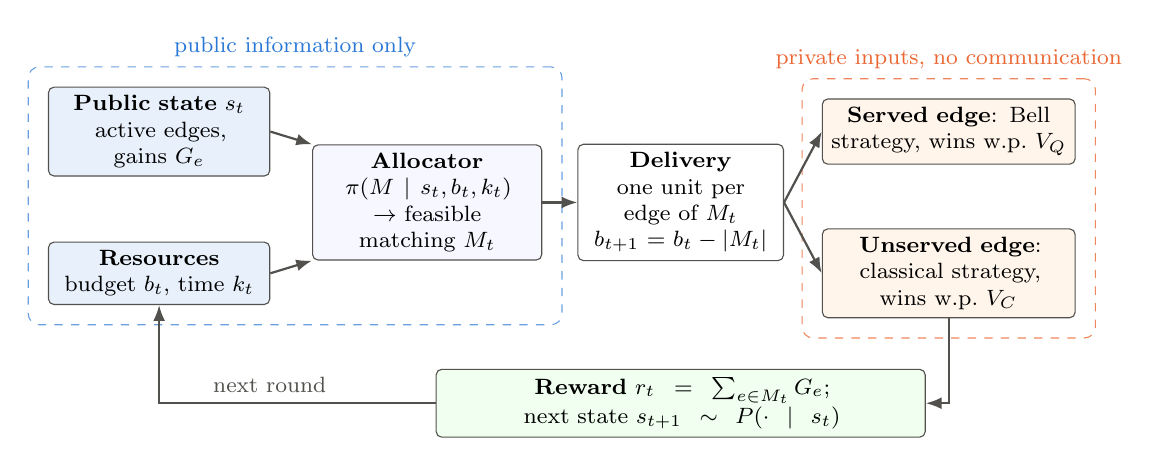
\begin{tikzpicture}[x=0.92cm,font=\footnotesize,
  box/.style={draw=inkgray,rounded corners=2pt,align=center,fill=white,inner sep=3pt},
  arr/.style={-{Latex[length=2mm]},thick,inkgray}]
\node[box,fill=softblue,text width=26mm] (state) at (0,0.9) {\textbf{Public state} $s_t$\\active edges, gains $G_e$};
\node[box,fill=softblue,text width=26mm] (res) at (0,-0.9) {\textbf{Resources}\\budget $b_t$, time $k_t$};
\node[box,fill=blue!3,text width=27mm] (alloc) at (3.7,0) {\textbf{Allocator}\\$\pi(M\mid s_t,b_t,k_t)$\\$\to$ feasible matching $M_t$};
\node[box,text width=24mm] (dist) at (7.2,0) {\textbf{Delivery}\\one unit per edge of $M_t$\\$b_{t+1}=b_t-|M_t|$};
\node[box,fill=orange!8,text width=30mm] (q) at (10.9,0.9) {\textbf{Served edge}: Bell strategy, wins w.p.\ $V_Q$};
\node[box,fill=orange!8,text width=30mm] (c) at (10.9,-0.9) {\textbf{Unserved edge}: classical strategy, wins w.p.\ $V_C$};
\node[box,fill=green!6,text width=60mm] (rew) at (7.2,-2.55) {\textbf{Reward} $r_t=\sum_{e\in M_t}G_e$; next state $s_{t+1}\sim P(\cdot\mid s_t)$};
\draw[arr] (state.east) -- (alloc.north west);
\draw[arr] (res.east) -- (alloc.south west);
\draw[arr] (alloc) -- (dist);
\draw[arr] (dist.east) -- (q.west);
\draw[arr] (dist.east) -- (c.west);
\draw[arr] (c.south) |- (rew.east);
\draw[arr] (rew.west) -| node[pos=0.3,above]{next round} (res.south);
\begin{scope}[on background layer]
\node[draw=ppoblue!70,dashed,rounded corners,fit=(state)(res)(alloc),inner sep=2.5mm] (pub) {};
\node[draw=dqnorange!80,dashed,rounded corners,fit=(q)(c),inner sep=2.5mm] (priv) {};
\end{scope}
\node[anchor=south,text=ppoblue] at (pub.north) {public information only};
\node[anchor=south,text=dqnorange] at (priv.north) {private inputs, no communication};
\end{tikzpicture}
\caption{One round of \bellroute{}. The allocator sees only public information and chooses a matching under the remaining budget. Each served edge consumes one unit.}
\label{fig:overview}
\end{figure}

\subsection{Splits, transfer, and resource noise}\label{sec:splits}

Request types were generated independently per split (18 development, 12 validation, and 16 test types), with disjoint identifiers and contents. Eight development and four validation catalogs cover three to six agents on path, ring, star, complete, and sparse graphs. The four sealed test catalogs are listed below. Catalogs marked $^\dagger$ share their public dynamics with a development catalog (\cref{sec:audit}).
\begin{itemize}[leftmargin=*]
  \item a four-agent complete graph with fresh requests$^\dagger$ ($H=10$, $B=6$);
  \item an unseen six-agent ring ($H=16$, $B=6$);
  \item an unseen eight-agent sparse graph with 11 edges ($H=24$, $B=10$);
  \item a four-agent path with a long horizon$^\dagger$ ($H=24$, $B=6$).
\end{itemize}
Two optional imperfections are modelled. Under \emph{Werner noise} with visibility $v$, the Bell value becomes $\tfrac12+v(V_Q-\tfrac12)$. Under \emph{heralded loss}, each attempted unit succeeds with probability $p_h$ and is consumed either way.

\subsection{Interface}\label{sec:gym}

\bellroute{} is a Gymnasium environment. Observations hold per-edge gains, active and present masks, endpoints padded to 28 edge slots, the remaining budget, and the remaining time. Actions are an index into a fixed enumeration of at most 407 matchings, with a feasibility mask in \texttt{info}. Episodes terminate at the horizon. The environment passes the Gymnasium environment checker. Under fixed seeds, it reproduces the archived evaluator's state sequences, heralding draws, and returns exactly in our unit tests.

%======================================================================
\section{Allocators}\label{sec:methods}
%======================================================================

All methods act on the same feasible sets and the same paired evaluation sequences. \Cref{tab:fairness} states what each one observes.

\paragraph{Learned allocators.} DQN \citep{mnih2015human}, Double DQN \citep{vanhasselt2016deep}, PPO \citep{schulman2017proximal}, and recurrent PPO (with a GRU, \citealp{cho2014learning}) share one permutation-invariant edge encoder \citep{zaheer2017deep} that supports up to eight agents. Each feasible matching $M$ is scored from per-edge features $(10G_e,\mathbf 1[e\text{ active}],\mathbf 1[e\in M])$, mean-pooled through a width-64 two-layer network. Eight global features are appended: $b/B$, $k/H$, $n/8$, $|M|/2$, $10G(M)$, and the maximum, mean, and count of current gains. Infeasible matchings are never scored. Each method was tuned over three (width, learning-rate) configurations with two seeds on development data. All selected width 64 and learning rate $10^{-3}$. Details are in \cref{app:training}.

\paragraph{Non-learned baselines registered with the locked study.} \emph{Random} samples a feasible matching uniformly. \emph{Static} uses fixed per-edge-index priorities from training gains. \emph{Greedy} maximizes the current $\sum_{e\in M}G_e$ (ties go to more pairs).

\paragraph{Comparators added after the locked study.} We added two comparators after the locked study, registered before they were run.
\begin{itemize}[leftmargin=*]
  \item \emph{Bid-price threshold.} For each state, take the edge gains of the best two-pair matching. Pool these ``slot gains'' from the training catalogs into a reference distribution with total weight $\omega$, and add every slot gain observed so far in the current episode with weight one. In round $t$, set the threshold $\theta_t$ to the $1-\alpha b_t/(2k_t)$ quantile of this mixture, or to zero if $\alpha b_t\ge 2k_t$. Then serve the best feasible matching whose every edge has $G_e\ge\theta_t$ and $G_e>0$. The rule spends freely when budget is plentiful relative to time and becomes selective as the budget tightens. This is the logic of bid-price control \citep{gallego1994optimal,talluri2004theory}. It has two parameters, $(\alpha,\omega)$, and never sees $P$.
  \item \emph{Certainty-equivalent DP (CE-DP).} Estimate $P$ from $K$ logged public state sequences of the catalog, as the posterior mean under a Dirichlet prior. The prior puts mass $\rho$ on staying in the current state and spreads the rest uniformly, with total mass $\kappa$, and $\rho$ is the mean self-loop probability of the development catalogs. Then solve the finite-horizon Bellman recursion exactly on the estimate \citep{bertsekas2017dynamic}. CE-DP requires the catalog's public state table and, for $K>0$, logged data from the test catalog. The learners receive neither, so CE-DP is an informed reference rather than an equal-information competitor.
\end{itemize}

\paragraph{References.} \emph{Online DP} knows the true $P$ and is the optimal non-anticipative policy. The \emph{future-clairvoyant} reference knows the realized state sequence. We report surplus as a fraction of online DP throughout.

\begin{table}[t]
\centering
\caption{Information available to each allocator. No method observes the endpoints' private inputs.}
\label{tab:fairness}
\small
\begin{tabularx}{\textwidth}{@{}l>{\raggedright\arraybackslash}X>{\raggedright\arraybackslash}p{40mm}@{}}
\toprule
Method & Observes beyond current gains, budget, and time & Fitted or tuned on \\
\midrule
Random, Greedy & nothing (random: not even gains) & --- \\
Static & fixed per-edge-index priorities & training-catalog gains \\
DQN, Double DQN, PPO, Rec.\ PPO & graph size; edge activity (rec.\ PPO: memory) & 12 training catalogs; 3 configs $\times$ 2 seeds \\
\textbf{Bid-price} & slot gains seen earlier in the episode & training gains; \bpConfigs{} configs on validation \\
\textbf{CE-DP} ($K$ sequences) & public state table and state identity; $K$ logged test-catalog sequences & $\rho$ from development; $\kappa$ on validation \\
Online DP & true transition matrix $P$ & --- \\
Future-clairvoyant & realized future states & --- \\
\bottomrule
\end{tabularx}
\end{table}

%======================================================================
\section{Protocol}\label{sec:protocol}
%======================================================================

The work ran in phases. Each phase committed and published its code, configuration, and hash-locked inputs before execution, and archived its raw records as hash-inventoried bundles.
\begin{enumerate}[leftmargin=*]
  \item Splits were generated and the test split hash-locked.
  \item Learners were tuned and ablated on development and validation data.
  \item Robustness and scaling were measured on validation data, and the confirmatory design was frozen.
  \item The sealed test split was opened once for the locked study.
  \item An independent audit re-derived every number from raw rows.
  \item The comparators of \cref{sec:methods} were added.
\end{enumerate}

\paragraph{Locked study design.} The locked study trained 12 fresh DQN and 12 fresh PPO models for 2{,}500 episodes each, on all 12 development and validation catalogs. Only final checkpoints were evaluated, on 500 paired sequences per sealed catalog. The unit of analysis is the training seed. A seed's score is its mean surplus, averaged with equal weight over catalogs. The three registered primary tests were:
\begin{enumerate}[leftmargin=*]
  \item PPO superior to DQN: the 95\% interval of the paired difference lies above 0;
  \item PPO superior to greedy;
  \item PPO--DQN equivalence: the 90\% interval lies inside $\pm5\%$ of the online-DP mean.
\end{enumerate}
Intervals are percentile bootstraps over seeds with 20{,}000 resamples \citep{efron1993introduction}. Secondary per-catalog contrasts use exact Wilcoxon signed-rank tests \citep{wilcoxon1945individual} with Holm adjustment \citep{holm1979simple}.

\paragraph{Post-lock comparator design.} The comparator run was registered with its decision rule before execution.
\begin{itemize}[leftmargin=*]
  \item \emph{Primary test:} PPO minus bid-price on the four sealed catalogs, with a seed bootstrap as above. The outcome is ``learned superior'' if the 95\% lower bound is $>0$, ``bid-price superior'' if the upper bound is $<0$, and inconclusive otherwise.
  \item \emph{Secondary analyses:} the same contrast for DQN and on the fresh-only catalogs. CE-DP is descriptive, and we report the smallest $K$ at which it reaches the PPO mean.
  \item \emph{Tuning:} both comparators were tuned on the four validation catalogs only (500 sequences each), over \bpConfigs{} bid-price and \ceConfigs{} CE-DP configurations. The code writes the selection to disk before reading any sealed file.
  \item \emph{Learned rows:} these are read from the locked study's archive. No model is retrained, reselected, or re-run.
  \item \emph{Evaluator check:} the comparator run first re-evaluated greedy and online DP and reproduced the archived rows exactly (maximum absolute error \reproErr).
\end{itemize}
These comparators were evaluated after the test split had been opened. They never informed any locked-study decision, and they had no access to test data before their single evaluation.

%======================================================================
\section{Results}\label{sec:results}
%======================================================================

\subsection{Locked study: learners beat greedy and are equivalent to each other}\label{sec:locked}

All 24 models completed without budget or matching violations. The three registered tests resolved as follows (\cref{tab:main}).
\begin{itemize}[leftmargin=*]
  \item \emph{PPO superior to greedy: supported.} The difference was $\ppoMinusGreedy$, with 95\% CI $[\ppoMinusGreedyLo,\ppoMinusGreedyHi]$, and all 12 seeds were ahead.
  \item \emph{PPO superior to DQN: not supported.} The difference was $\ppoMinusDqn$, with 95\% CI $[\ppoMinusDqnLoNinetyFive,\ppoMinusDqnHiNinetyFive]$.
  \item \emph{PPO--DQN equivalence: supported.} The 90\% CI $[\ppoMinusDqnLoNinety,\ppoMinusDqnHiNinety]$ lies within $\pm\eqMargin$.
\end{itemize}
No per-catalog PPO--DQN contrast survived Holm adjustment (\cref{app:secondary}). The learners recovered \fracPPO\% (PPO) and \fracDQN\% (DQN) of the online-DP surplus, against \fracGreedy\% for greedy. They transferred to the unseen eight-agent graph without retraining. In development, the four learners were within $0.02$ of each other, and the registered hypothesis that Double DQN would be best was not supported (\cref{app:training}). Taken alone, these results would support a conventional conclusion: deep RL learns resource-aware allocation that transfers across graphs and roughly halves the gap between greedy and optimal.

\begin{table}[t]
\centering
\caption{Mean surplus on the sealed catalogs; parentheses give the percentage of online-DP surplus. Learned rows average 12 seeds $\times$ 500 sequences. Other rows use the same 500 sequences. Bid-price and CE-DP (post-lock comparators, tuned on validation only) are below the rule. $^\dagger$Public dynamics shared with a development catalog.}
\label{tab:main}
\small
\setlength{\tabcolsep}{4pt}
\begin{tabular}{@{}lccccc@{}}
\toprule
Method & \shortstack{4-agent\\complete$^\dagger$} & \shortstack{6-agent\\ring} & \shortstack{8-agent\\sparse} & \shortstack{4-agent path\\$H{=}24^\dagger$} & Overall \\
\midrule
Random & \catCmpRandom & \catRingRandom & \catSparseRandom & \catPathRandom & \meanRandom \\
Static & \catCmpStatic & \catRingStatic & \catSparseStatic & \catPathStatic & \meanStatic \\
Greedy & \catCmpGreedy{} (\fracCmpGreedy) & \catRingGreedy{} (\fracRingGreedy) & \catSparseGreedy{} (\fracSparseGreedy) & \catPathGreedy{} (\fracPathGreedy) & \meanGreedy{} (\fracGreedy) \\
DQN & \catCmpDQN{} (\fracCmpDQN) & \catRingDQN{} (\fracRingDQN) & \catSparseDQN{} (\fracSparseDQN) & \catPathDQN{} (\fracPathDQN) & \meanDQN{} (\fracDQN) \\
PPO & \catCmpPPO{} (\fracCmpPPO) & \catRingPPO{} (\fracRingPPO) & \catSparsePPO{} (\fracSparsePPO) & \catPathPPO{} (\fracPathPPO) & \meanPPO{} (\fracPPO) \\
\midrule
\textbf{Bid-price} & \textbf{\catCmpBp} (\fracCmpBp) & \textbf{\catRingBp} (\fracRingBp) & \textbf{\catSparseBp} (\fracSparseBp) & \textbf{\catPathBp} (\fracPathBp) & \textbf{\bpMean} (\bpFrac) \\
CE-DP, $K{=}0$ & \catCmpCeZero{} (\fracCmpCeZero) & \catRingCeZero{} (\fracRingCeZero) & \catSparseCeZero{} (\fracSparseCeZero) & \catPathCeZero{} (\fracPathCeZero) & \ceZeroMean{} (\ceZeroFrac) \\
\midrule
Online DP (true $P$) & \catCmpOnline & \catRingOnline & \catSparseOnline & \catPathOnline & \meanOnline \\
Future-clairvoyant & \catCmpFuture & \catRingFuture & \catSparseFuture & \catPathFuture & \meanFuture \\
\bottomrule
\end{tabular}
\end{table}

\subsection{Strong baselines withdraw the learned claim}\label{sec:strong}

Validation tuning selected bid-price parameters $\alpha=\bpAlpha$ and $\omega=\bpPrior$, with a validation mean of \bpValMean. The landscape is smooth, and a broad region of the grid performs similarly (\cref{fig:tuning}a). On the sealed catalogs, the registered primary contrast resolved \emph{bid-price superior}.
\begin{itemize}[leftmargin=*]
  \item \emph{All catalogs:} PPO minus bid-price was $\ppoMinusBp$ (95\% CI $[\ppoMinusBpLo,\ppoMinusBpHi]$), and none of the 12 PPO seeds was ahead. DQN minus bid-price was $\dqnMinusBp$ ($[\dqnMinusBpLo,\dqnMinusBpHi]$).
  \item \emph{Fully fresh catalogs only:} PPO minus bid-price was $\frppoMinusBp$ ($[\frppoMinusBpLo,\frppoMinusBpHi]$), and DQN minus bid-price was $\frdqnMinusBp$ ($[\frdqnMinusBpLo,\frdqnMinusBpHi]$).
\end{itemize}
The heuristic reached \bpFrac\% of online DP overall and between \fracSparseBp\% and \fracPathBp\% on every catalog (\cref{tab:main,fig:fraction}). The registered falsifier for the learned claim therefore fired. The learned allocators beat greedy, but a two-parameter rule that never sees the dynamics beats them on every seed and every catalog. Measured against the online-DP optimum, the heuristic closes \gapClosed\% of the gap that PPO leaves.

CE-DP was within $0.5\%$ of online DP at every registered data size, ranging from \ceFracMin\% to \ceFracMax\% (\cref{fig:tuning}b). Even with $K=0$, which uses no test-catalog transitions, only the state table and a generic self-loop prior, it reached \ceZeroFrac\%. The registered break-even data size is therefore $K=0$: CE-DP needs no logged dynamics to beat both learners (PPO minus CE-DP was $\ppoMinusCeZero$, with 95\% CI $[\ppoMinusCeZeroLo,\ppoMinusCeZeroHi]$).

\begin{figure}[t]
\centering
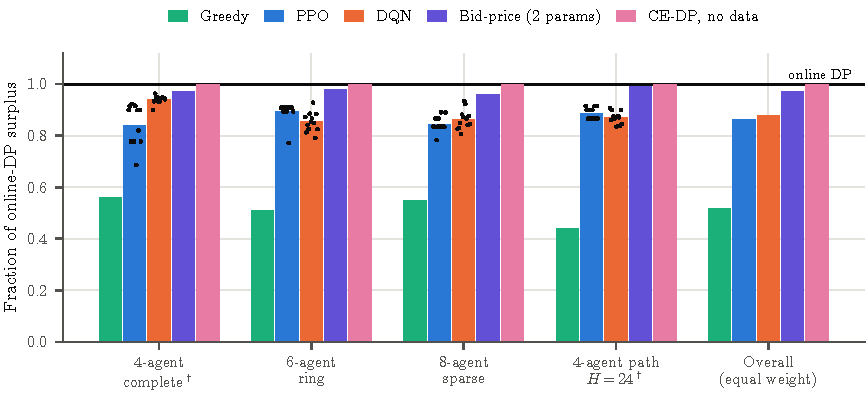
\includegraphics[width=\textwidth]{fig_fraction_online.pdf}
\caption{Fraction of the online-DP surplus on each sealed catalog. Dots are the 12 individual PPO and DQN training seeds. Bid-price and CE-DP ($K=0$) were tuned on validation data only and evaluated once. Source data: \texttt{tmlr\_fraction\_online.csv}.}
\label{fig:fraction}
\end{figure}

\begin{figure}[t]
\centering
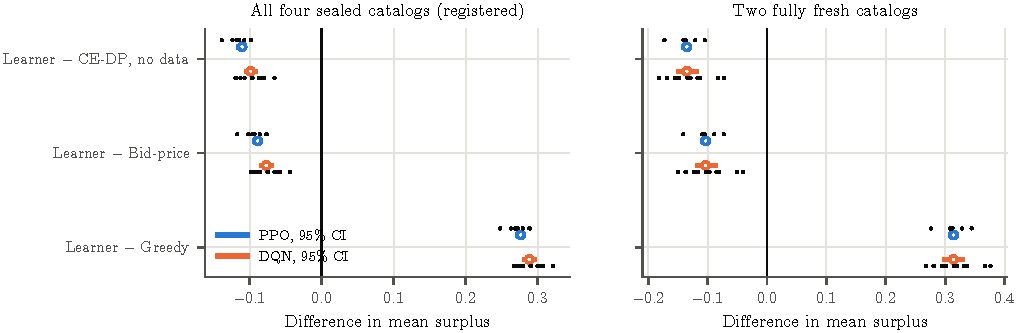
\includegraphics[width=\textwidth]{fig_contrasts.pdf}
\caption{Seed-level contrasts with 95\% percentile bootstrap intervals (20{,}000 resamples). Small dots are individual training seeds. Learners beat greedy on every seed but lose to bid-price and CE-DP on every seed, both on all catalogs (left; registered) and on the two fully fresh catalogs (right). Source data: \texttt{tmlr\_contrasts.csv}, \texttt{tmlr\_seed\_contrasts.csv}.}
\label{fig:contrasts}
\end{figure}

\begin{figure}[t]
\centering
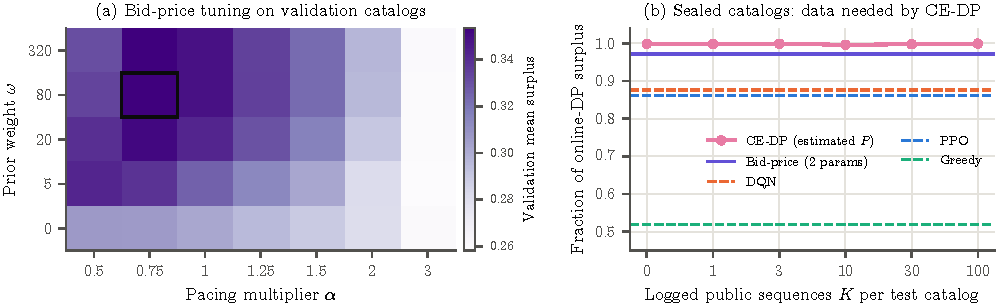
\includegraphics[width=\textwidth]{fig_tuning_ce.pdf}
\caption{\emph{(a)} Validation-only tuning landscape of the bid-price rule, with the selected cell outlined. $\omega=0$ uses only gains observed in the current episode. \emph{(b)} On the sealed catalogs, certainty-equivalent DP matches online DP at every amount of logged data, including none. Horizontal lines are the other methods. Source data: \texttt{tmlr\_tuning\_bid\_price.csv}, \texttt{tmlr\_ce\_dp\_test.csv}.}
\label{fig:tuning}
\end{figure}

\subsection{Why the simple rules win}\label{sec:why}

Three observations locate the learners' shortfall. They are diagnostic, not confirmatory.

\paragraph{Dynamics are nearly irrelevant; pacing is not.} CE-DP with a generic prior is as good as DP with the true $P$. So knowing \emph{how} demand evolves is worth almost nothing here. Knowing \emph{what} gains can appear (the state table) and how many units remain is worth almost everything. The bid-price rule estimates the gain distribution from training catalogs and the current episode, which is enough to reach 97\%. The learners must infer the same pacing behaviour from 2{,}500 episodes of reward signal. They reach 86--88\%.

\paragraph{The development ablations agree.} Removing the remaining-budget feature from Double DQN cost \ablDropNoBudget\% of validation surplus, and removing remaining time cost \ablDropNoHorizon\% (\cref{app:training}). These two inputs are exactly the quantities that set the bid-price threshold. The learners use them, but less precisely than a closed-form quantile rule.

\paragraph{The gap was visible before the test split.} On validation catalogs, the selected bid-price rule scored \bpValMean, while the four tuned learners scored \develRPPO--\develPPO{} in development (on different sequences of the same catalogs). Had the bid-price rule been in the original baseline set, the learned claim would most likely not have been registered as the primary hypothesis.

\paragraph{Learner limitations we cannot rule out.} The learners' tuning grid was small, and the selected configuration sat at its edge (the largest learning rate tried). Training was short, and PPO's value head was not calibrated to the advantage scale (\cref{app:training}). Also, 12 PPO seeds collapsed onto \ppoDistinctSeedValues{} distinct outcomes. Better-tuned or longer-trained learners might close part of the gap. Our claim is narrower: under a preregistered, equal-opportunity protocol, the learners did not, and a two-parameter rule did.

\subsection{Transfer and the fully fresh catalogs}\label{sec:transfer}

On the two fully fresh catalogs (the unseen six-agent ring and eight-agent sparse graph), PPO and DQN each kept \ppoFracFresh\% of online DP, greedy kept \greedyFracFresh\%, and bid-price kept \bpFracFresh\%. All qualitative conclusions are unchanged when the two catalogs with leaked dynamics are excluded (\cref{fig:contrasts}, right).

\subsection{Resource noise and a fidelity threshold}\label{sec:noise}

Under heralded loss, the learned surplus scaled proportionally with $p_h$. PPO kept \ratioHerSevenFive{} of its ideal surplus at $p_h=0.75$ and \ratioHerFive{} at $p_h=0.5$. Under Werner noise, the surplus of every method vanished at $v\le0.8$. This is a property of the request family, not of the allocators. A request keeps a positive gain only if $v>v^*(\tau)=(V_C-\tfrac12)/(V_Q-\tfrac12)$. On the sealed family $v^*$ has minimum \thrTestMin{} and median \thrTestMedian. Of the sealed state-table entries, \posOppIdeal\% carry a positive gain with ideal pairs, \posOppNine\% at $v=0.9$, and none at $v=0.8$ (\cref{app:noise}). For RL purposes, the noisy variants change the reward scale and sparsity rather than the decision structure. Users of the benchmark should report results at stated $v$ and $p_h$.

%======================================================================
\section{Audit and reproducibility}\label{sec:audit}
%======================================================================

A separate audit module re-derived every locked-study quantity from the raw episode rows, independently of the analysis code, the environment, and the learners. It reproduced all means, intervals, $p$-values, Holm adjustments, and thresholds to within $10^{-9}$. It re-certified every sealed request with an independently formulated SDP solved with CVXPY \citep{diamond2016cvxpy}. It verified checkpoint hashes, the split locks, and resource ledgers.

The audit also found a real defect. The catalog generator derived each catalog's seed from the split seed plus a small offset, so seeds collided across splits. As a result, two sealed test catalogs reuse the public \emph{dynamics} (transition matrix, active-edge pattern, urgencies) of development catalogs, although their request types are fresh. One validation catalog duplicates a development catalog in the same way. We kept the locked analysis as registered and report every result on the two fully fresh catalogs as well. None of the conclusions depends on the overlapping catalogs. The comparator run of \cref{sec:strong} added \wallThirty{} wall-seconds of single-thread CPU time and no training (\cref{app:compute}).

All code, configurations, hash-locked splits, raw records, checkpoints, and audit bundles are provided as anonymized supplementary material and will be released publicly. Every number and data figure in this paper is generated by scripts from these bundles.

%======================================================================
\section{Discussion and limitations}\label{sec:discussion}
%======================================================================

\paragraph{Lessons for evaluating RL on allocation problems.} In budgeted allocation, greedy is a straw man. It ignores the one quantity that matters most, the opportunity cost of a unit. Operations research has offered closed-form opportunity-cost rules for decades \citep{gallego1994optimal,talluri2004theory}. We suggest two practices that would have caught our overclaim at the development stage.
\begin{itemize}[leftmargin=*]
  \item Include at least one pacing or bid-price heuristic and one certainty-equivalent planner among the registered baselines.
  \item Report learners as a fraction of an exact or near-exact optimum, alongside the simple rules, so that ``86\% of optimal'' is read against ``97\% from two parameters.''
\end{itemize}
Preregistration did its job here: it made the negative result unambiguous and prevented post hoc re-framing. But preregistration cannot fix a weak baseline set chosen in advance.

\paragraph{What the benchmark is good for.} \bellroute{} remains useful precisely because its optimum is computable. Learners can be measured on an absolute scale, against strong simple rules, and under controlled distribution shift in graph size, horizon, budget, and resource noise. Natural harder variants would remove the structure that makes CE-DP easy. Examples are unknown or non-stationary state tables, partial observability of requests, decentralized allocation, and memory decoherence that makes saving units costly. A method that beats bid-price and CE-DP on such variants would be strong evidence for learning.

\paragraph{Limitations.}
\begin{itemize}[leftmargin=*]
  \item The study has 12 seeds per learner, four test catalogs, at most eight agents, and 14-state chains.
  \item The comparators were evaluated after the test split had been opened. They had no prior access to it and were registered before running, but this is weaker than inclusion in the original lock.
  \item Two test catalogs leak public dynamics (\cref{sec:audit}).
  \item Rewards are analytic expectations over private inputs; no game rounds are sampled.
  \item The learners' tuning budget was small, as noted in \cref{sec:why}.
  \item The quantum layer is idealized: single-hop links, Werner noise, and independent heralding, with no hardware.
\end{itemize}

%======================================================================
\section{Conclusion}\label{sec:conclusion}
%======================================================================

Four deep RL allocators, evaluated under a preregistered and audited protocol, beat greedy allocation of a scarce resource by a wide and precise margin and transferred to unseen graphs. A two-parameter bid-price rule beat all of them on every seed, and a planner with no logged dynamics was within $0.1\%$ of optimal. The most useful outputs of this work are therefore the benchmark, with its exact optimum, sealed splits, and Gymnasium interface, and the record of how a careful study can still overclaim when its baseline set is too weak.

\subsubsection*{Broader impact statement}
This work concerns resource allocation in simulated quantum networks and the methodology of RL evaluation. We do not foresee direct negative societal impacts. Its main practical message, to compare learned controllers with strong classical rules before deploying them, should reduce unnecessary complexity in deployed allocation systems.

\subsubsection*{Use of AI tools}
The experiment code, analysis, audit, and drafts of this manuscript were produced with AI coding assistants operating under the authors' direction within a recorded, version-controlled protocol. The authors reviewed the work and take responsibility for its content.

\bibliography{references}
\bibliographystyle{tmlr}

\appendix

%======================================================================
\section{Learner training, development results, and ablations}\label{app:training}
%======================================================================

\paragraph{Training.}
\begin{itemize}[leftmargin=*]
  \item \emph{DQN:} a 20{,}000-transition replay buffer, minibatches of 64, the Huber loss, the undiscounted finite-horizon target $10r_t+\mathbf 1[t<H]\max_{M'}Q_{\bar\theta}$, target copies every 200 updates, and $\varepsilon$ decaying linearly from 1 to 0.03 over the first 65\% of episodes. Double DQN decouples selection from evaluation \citep{vanhasselt2016deep}.
  \item \emph{PPO:} rollouts of 16 episodes, then 4 epochs of the clipped objective (clip 0.2, value coefficient 0.5, entropy 0.01) with Monte Carlo returns. As frozen, its value head regresses standardized returns while the advantage subtracts its raw output from unstandardized returns, so it acts as a state-dependent offset rather than a calibrated baseline. Recurrent PPO adds a width-64 GRU that is reset at episode start.
  \item \emph{Shared settings:} all learners use Adam \citep{kingma2015adam} with gradient clipping at 5 and reward scale 10. DQN has \paramsDQN{} parameters, and PPO has \paramsPPO{} (policy plus value).
\end{itemize}

\paragraph{Development configurations.} DQN and Double DQN tried (width, learning rate) $\in\{(32,3{\times}10^{-4}),(64,3{\times}10^{-4}),(64,10^{-3})\}$. PPO and recurrent PPO tried $\{(32,10^{-4}),(64,3{\times}10^{-4}),(64,10^{-3})\}$. Each configuration had two seeds and 1{,}200 episodes, and selection used the final checkpoint on 300 validation sequences per catalog. Validation means were DQN \develDQN, Double DQN \develDDQN, PPO \develPPO, and recurrent PPO \develRPPO. The registered Double-DQN superiority hypothesis was not supported (difference from PPO: $\develDDQNMinusPPO$).

\paragraph{Ablations (Double DQN, validation).} Starting from \develDDQN{} with the full input set:
\begin{itemize}[leftmargin=*]
  \item no remaining-budget input: \ablNoBudget{} ($-$\ablDropNoBudget\%);
  \item binary instead of real-valued gains: \ablBinary{} ($-$\ablDropBinary\%);
  \item gains shuffled across active edges: \ablShuffled{} ($-$\ablDropShuffled\%);
  \item no remaining-time input: \ablNoHorizon{} ($-$\ablDropNoHorizon\%).
\end{itemize}
\Cref{fig:ablation} shows these results.

\begin{figure}[H]
\centering
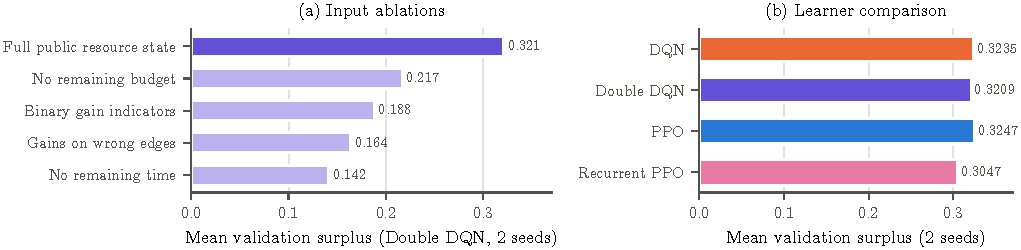
\includegraphics[width=\textwidth]{fig_ablation.pdf}
\caption{Development results on validation catalogs. \emph{(a)} Input ablations of Double DQN. \emph{(b)} The four tuned learners.}
\label{fig:ablation}
\end{figure}

\paragraph{An earlier single-graph study.} A precursor study on one four-agent complete graph (16 seeds, 1{,}000 test sequences) gave a learned-minus-greedy difference of \sOneDiff{} (95\% CI [\sOneDiffLo, \sOneDiffHi]) and \sOneFrac\% of online DP. Its preregistered gate required a 95\% lower bound of at least 90\% of online DP, and it \emph{failed}, with a lower bound of \sOneFracLo\%.

%======================================================================
\section{Secondary locked-study contrasts}\label{app:secondary}
%======================================================================

\begin{table}[H]
\centering
\caption{Per-catalog PPO$-$DQN contrasts: exact one-sided Wilcoxon signed-rank tests over 12 seed pairs, Holm-adjusted over four catalogs.}
\small
\begin{tabular}{@{}lrrr@{}}
\toprule
Catalog & PPO $-$ DQN & PPO seed wins & raw $p$ / Holm $p$ \\
\midrule
4-agent complete & \diffCmp & \winsCmp/12 & \rawpCmp{} / \holmpCmp \\
6-agent ring & \diffRing & \winsRing/12 & \rawpRing{} / \holmpRing \\
8-agent sparse & \diffSparse & \winsSparse/12 & \rawpSparse{} / \holmpSparse \\
4-agent path, $H=24$ & \diffPath & \winsPath/12 & \rawpPath{} / \holmpPath \\
\bottomrule
\end{tabular}
\end{table}

%======================================================================
\section{Resource noise}\label{app:noise}
%======================================================================

\begin{table}[H]
\centering
\caption{Mean surplus under resource imperfections. Validation rows: three seeds per learner and four validation catalogs. Sealed-test row: 12 PPO models on the first 100 sequences per catalog.}
\small
\setlength{\tabcolsep}{4pt}
\begin{tabular}{@{}lcccccccc@{}}
\toprule
& Ideal & $p_h{=}0.9$ & $p_h{=}0.75$ & $p_h{=}0.5$ & $v{=}0.9$ & $v{=}0.8$ & $v{=}0.7$ & $v{=}0.6$ \\
\midrule
DQN (val.) & \validDQNIdeal & \validDQNHerNine & \validDQNHerSevenFive & \validDQNHerFive & \validDQNVisNine & \validDQNVisEight & \validDQNVisSeven & \validDQNVisSix \\
Double DQN (val.) & \validDDQNIdeal & \validDDQNHerNine & \validDDQNHerSevenFive & \validDDQNHerFive & \validDDQNVisNine & \validDDQNVisEight & \validDDQNVisSeven & \validDDQNVisSix \\
PPO (val.) & \validPPOIdeal & \validPPOHerNine & \validPPOHerSevenFive & \validPPOHerFive & \validPPOVisNine & \validPPOVisEight & \validPPOVisSeven & \validPPOVisSix \\
Rec.\ PPO (val.) & \validRPPOIdeal & \validRPPOHerNine & \validRPPOHerSevenFive & \validRPPOHerFive & \validRPPOVisNine & \validRPPOVisEight & \validRPPOVisSeven & \validRPPOVisSix \\
\midrule
PPO (sealed) & \noiseIdealHundred & -- & \noiseHerSevenFive & \noiseHerFive & -- & \noiseVisEight & -- & \noiseVisSix \\
\bottomrule
\end{tabular}
\end{table}

\begin{figure}[H]
\centering
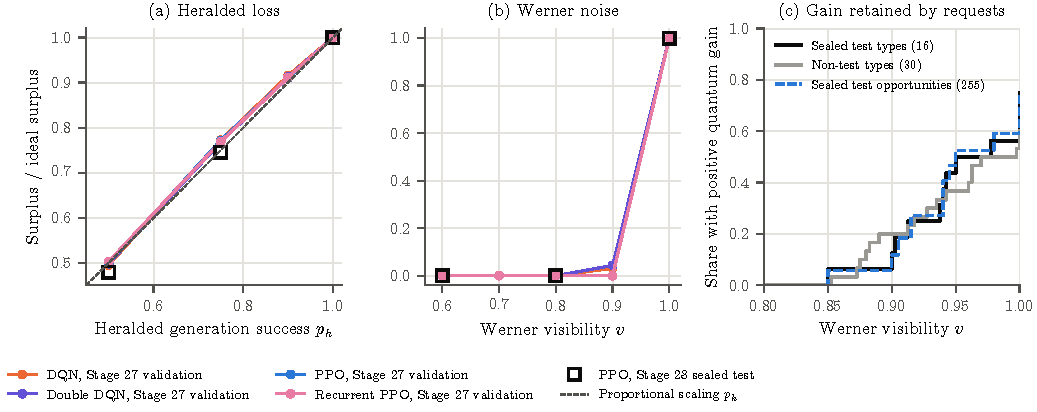
\includegraphics[width=\textwidth]{fig_noise.pdf}
\caption{\emph{(a)} Heralded loss scales surplus proportionally. \emph{(b)} Werner noise removes it at $v\le0.8$. \emph{(c)} The share of request types and sealed occurrences with a positive gain at visibility $v$.}
\end{figure}

%======================================================================
\section{Compute}\label{app:compute}
%======================================================================

The locked study used \resDecisions{} allocator decisions and \resWallHours{} active wall-hours on one CPU thread (cap 4\,h). It ran no GPU and sampled no shots. Across the development, robustness, and locked phases, the work used \progDecisions{} decisions and \progWallHours{} wall-hours. The comparator run used \decisionsThirty{} decisions, \wallThirty{} wall-seconds, and \cpuThirty{} CPU core-hours, with no training. An earlier comparator attempt with identical configuration is retained in the archive. It produced identical results, but was rejected by the archive validator because of a stage-registry schema bug unrelated to the experiment.

\end{document}
